\documentclass[aspectratio=169]{beamer}
\usetheme{Madrid}
\usepackage[utf8]{inputenc}
\usepackage[T1]{fontenc}
\usepackage{tikz}
\usepackage{amssymb}
\usepackage{graphicx}
\setbeamertemplate{navigation symbols}{}
\setbeamercolor{title}{fg=white,bg=red!80!orange}
\setbeamercolor{frametitle}{fg=white,bg=red!80!orange}
\setbeamercolor{block title}{bg=red!80!orange!20,fg=black}
\setbeamercolor{block body}{bg=red!80!orange!8,fg=black}
\setbeamercolor{item}{fg=red!80!orange}
\setbeamercolor{itemize item}{fg=red!80!orange}
\setbeamertemplate{itemize item}[triangle]

\title{Phase 2 Tutorial — Your Code Fights}
\subtitle{A turn-based loop: read state, decide, act --- every single turn}
\author{ByteForge --- Grade 9 --- The Deep Diver}
\date{}

\begin{document}

\begin{frame}
    \titlepage
\end{frame}

\begin{frame}{Today's Missions}
    \Large
    \begin{itemize}
        \item First Contact
        \item Return Fire
    \end{itemize}
\end{frame}

\begin{frame}{Your code re-runs fresh, every single turn}
    \large
    \begin{itemize}
        \item Not write-once-run-once like the turtle missions
        \item Reads the LATEST \texttt{state} every turn --- your hp, the enemy, everything
        \item \texttt{attack(id)} or \texttt{wait()} --- whichever fires first is your move
    \end{itemize}
\end{frame}


\begin{frame}{This is a real, common program shape}
    \large
    \begin{itemize}
        \item "Loop forever: read the situation, decide, act"
        \item A game engine, a robot controller, even a thermostat all work this way
    \end{itemize}
\end{frame}


\begin{frame}{Hesitation has a real cost}
    \large
    \begin{itemize}
        \item An enemy that fights back changes everything
        \item \texttt{wait()} is not neutral if you are taking damage for free
        \item Read \texttt{state["self"]["hp"]} --- your OWN status matters too, not just the enemy's
    \end{itemize}
\end{frame}

\begin{frame}{Real-World Examples}
    \large
    \begin{itemize}
        \item A thermostat genuinely runs "read temperature, decide, act (heat or don't)" forever, exactly like this tier's battle loop.
    \end{itemize}
\end{frame}


\begin{frame}{Image}
    \begin{center}
    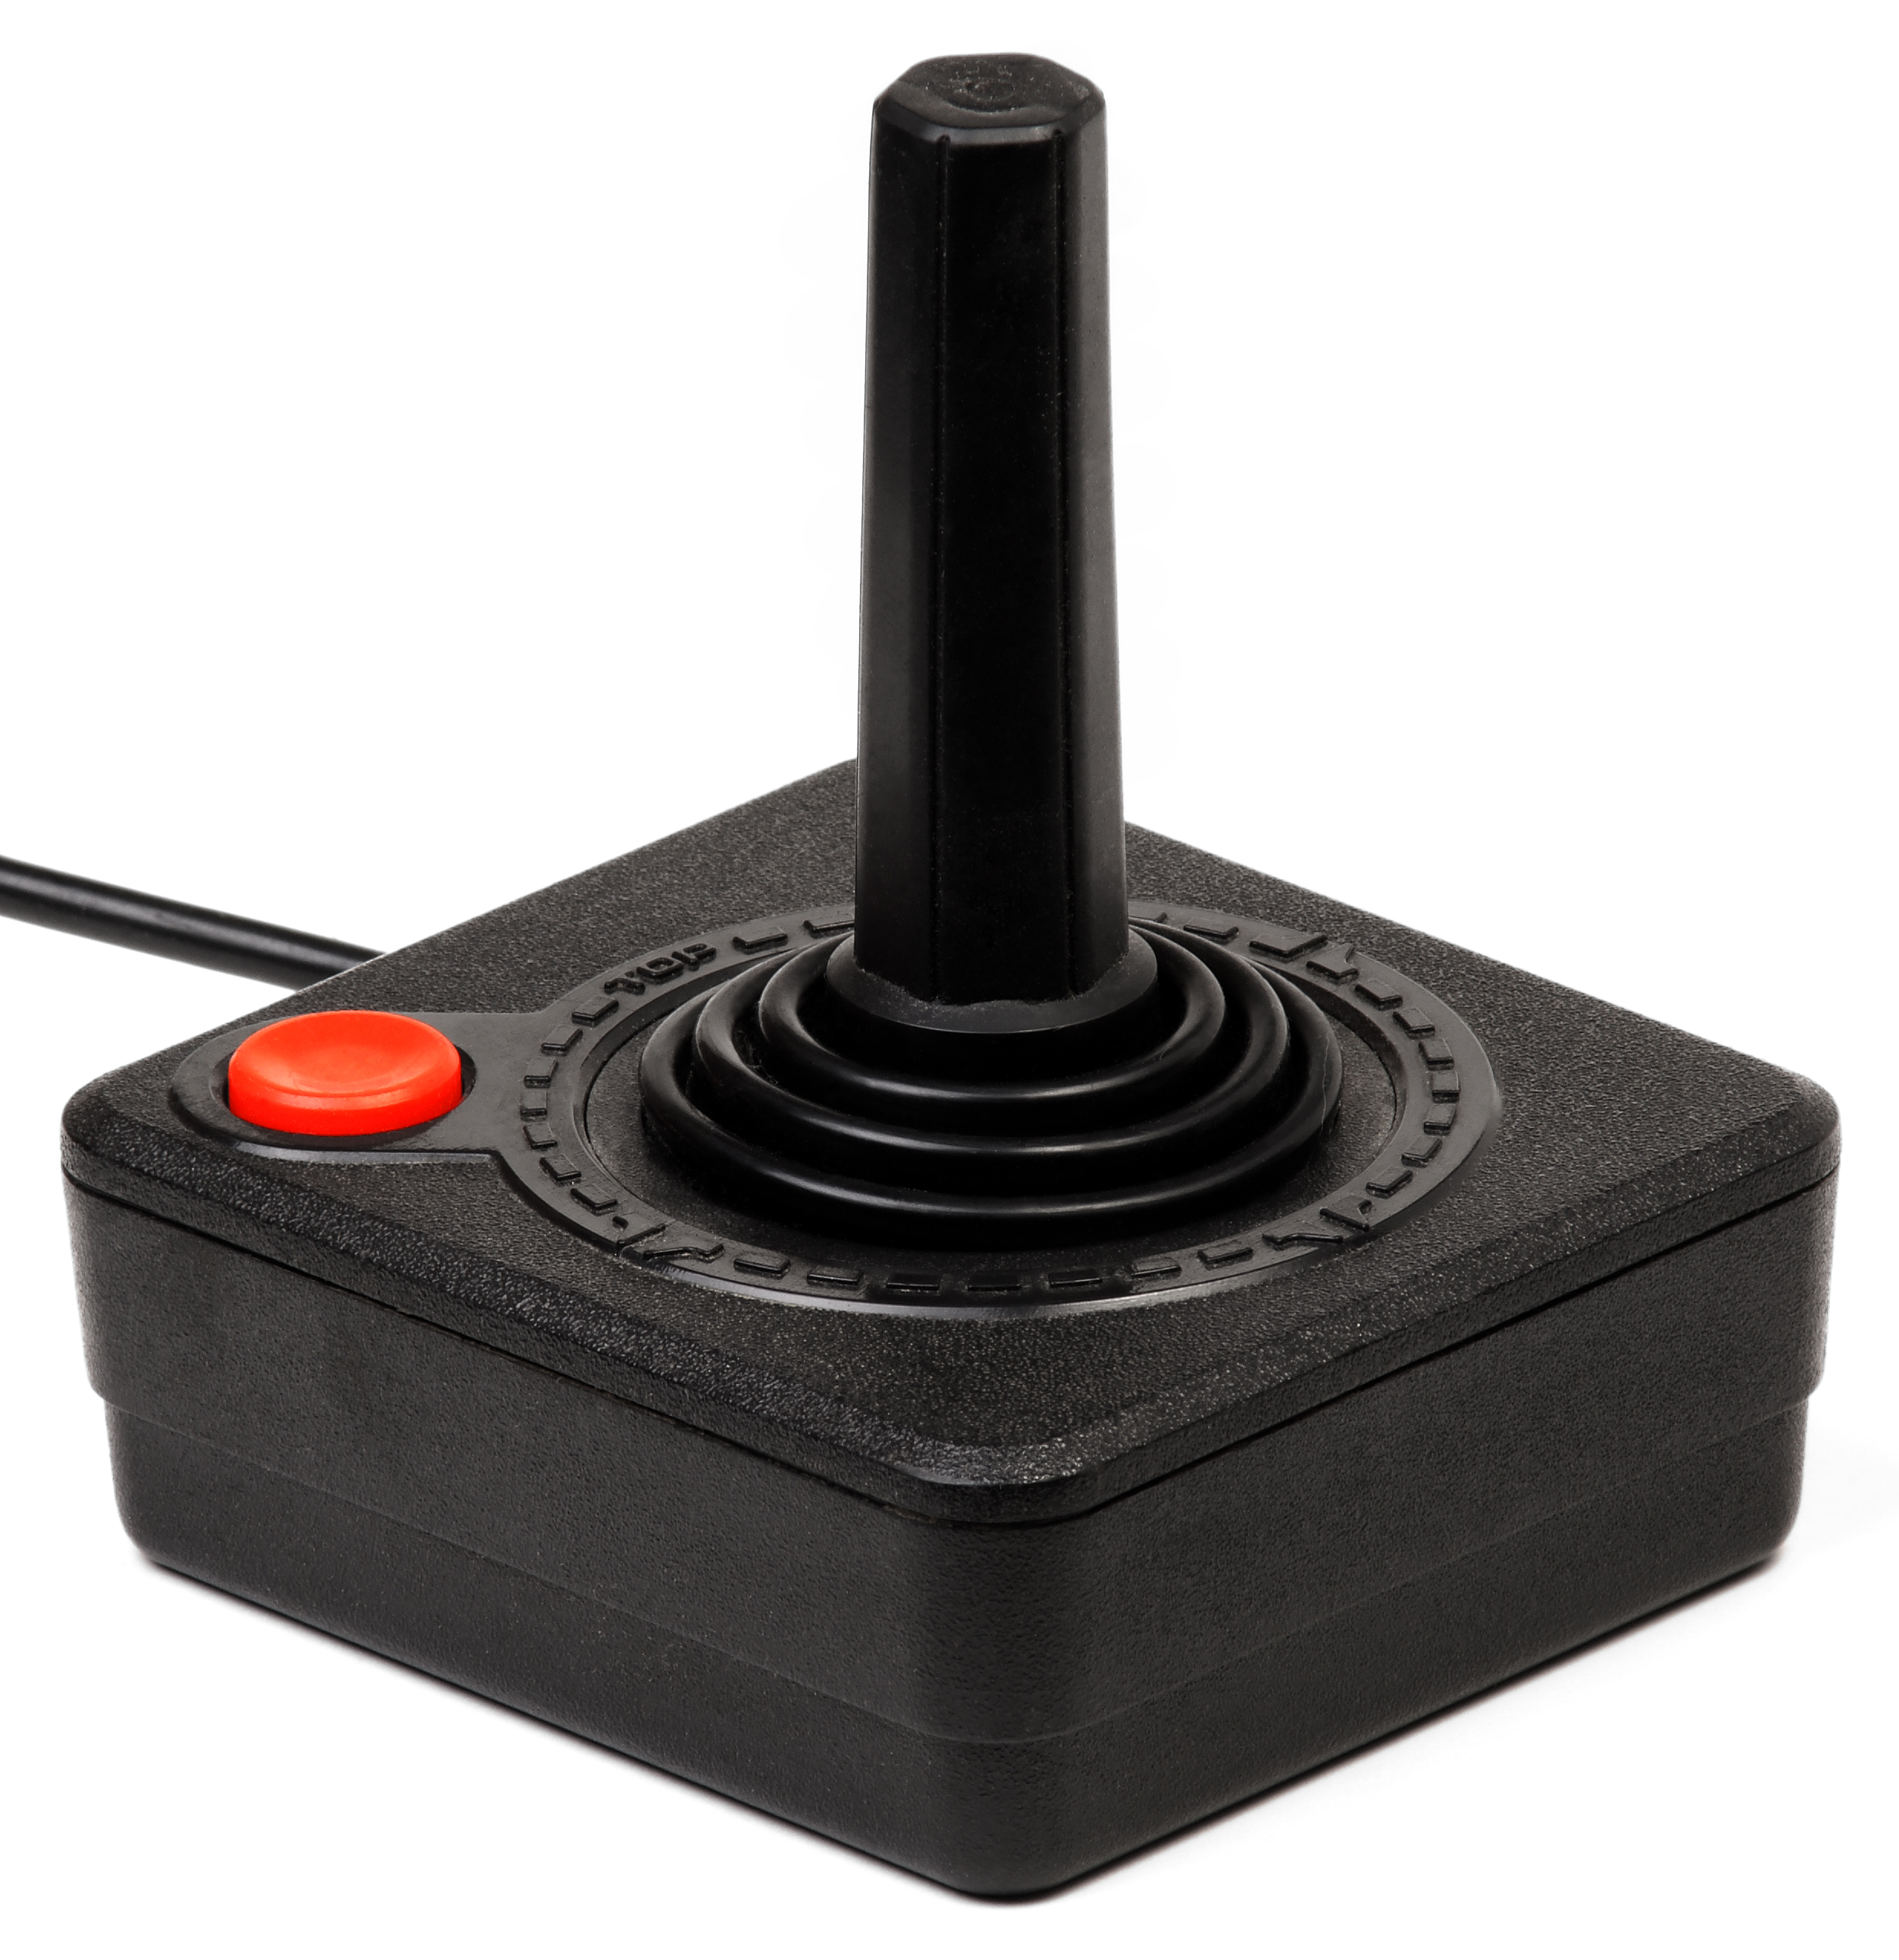
\includegraphics[width=0.5\textwidth]{images/joystick.jpg}

    \large This tier is a real turn-based fight --- read the situation, decide, act, exactly like a real game controller input loop.

    \small Atari 2600 joystick --- Evan-Amos, public domain, via Wikimedia Commons
    \end{center}
\end{frame}

\begin{frame}{Let Them Discover}
    \large
    Think of a real turn-based game you know (chess, a card game). What "state" would your code need to read before deciding its next move?
\end{frame}

\begin{frame}{Your Turn}
    \Large
    Open the mission map, find \textbf{Phase 2 Tutorial — Your Code Fights}, and fly it for real ---
    everything you just saw, you now do yourself.
\end{frame}

\end{document}
